\chapter{Related Work} \label{related_work}
Although DoH is relatively new compared to other security protocols, there is already a contemplative amount of work done in relation to DoH. The main focus of this chapter is to create an overview of the work which was already conducted concerning DoH. The first reference shows a study where they conducted downgrading Attacks on DoH connections in four different ways, followed by a reference which presents ways to detect and analyze DoH traffic by existing tools. All the following references show how machine learning or deep learning models can be used to detect malicious DoH traffic. The first reference shows that it is possible to separate DoH traffic from other traffic by using machine leanring models by first conducting a detailed feature analysis of DoH traffic and later different machine learning models. The second reference set the cornerstone for all the upcoming references by creating a data-set containing malicious and benign DoH traffic and non DoH traffic, including a feature extraction module. The next reference tried to separate malicious DoH traffic from benign traffic by using machine learning models. The fourth reference did essentially the same task but this time by using a layer-approach where he first separated DoH traffic from non-DoH traffic and then in the second layer separated benign DoH traffic from malicious traffic. He also tested several machine learning models. The fifth reference took the work of the fourth reference and improved it by conducting statistical tests for a more efficient feature extraction and machine learning model performance. The last reference in the machine learning Section designed a three-layered approach where they took the idea with the two-layers of the fourth reference and tried to find out which DoH tunnel tool was causing the malicious traffic in the third layer. The last reference in this chapter used deep learning approaches for the detection of malicious DoH traffic. In Table \ref{tab:summary} the key dimensions of every reference are summarized.

\section{Downgrading Attacks on DoH} \label{downgrading}
\cite{HuangEtAl_DoHDowngradeAttack} conducted a study where they carried out DoH downgrade attacks on six different browsers (Chrome, Firefox, Edge, Brave, Opera, and Vivaldi). A DoH downgrade attack translates DoH traffic into plain text DNS or in other words, the encrypted DoH connection is turned into a unencrypted DNS connection. DoH Communication has two phases: in the first phase the client connects for the first time with the resolver using an unencrypted DNS request and in the second phase a secure DoH connection is established and from this moment client and server only communicate with encrypted HTTPS GET and POST methods. In both phases, attackers who are able to intervene can keep the communication on the lower security level. \cite{HuangEtAl_DoHDowngradeAttack} proposed four different attack vectors during the two mentioned phases: DNS Traffic Interception, DNS Cache Poisoning, TCP Traffic Interception and TCP Reset Injection. They tested every combination of browser and attack vector and found that every single test lead to a successful attack. As countermeasures they proposed revisions of DoH implementations or DoH protocols.

\section{Capturing and Analyzing DoH Traffic} \label{capturing}
\cite{Hjelm_ANewNeedle} presented a study where he first conducted several tests to detect encrypted DNS traffic, especially DoH traffic. His goal was to show how attackers can use DoH to bypass the existing monitoring of organizations. Furthermore he proposed systems that is able to detect and restrain unintentional DoH traffic. He also presented Zeek, which can be used to observe the DNS traffic and record the traffic in Zeek logs, which can be passed to another tool called RITA. RITA can be used to interpret the Zeek logs statistically to identify malicious traffic such as beaconing. His findings are that companies can protect themselves by using and adequate analysis and monitoring setup.

\section{Machine Learning Based Approaches} \label{ml}
The references in this Section used ML based approaches. In the first reference the basis was built all the upcoming references by creating a data-set and an associated feature extraction. The further references evaluated different ways to detect malicious DoH traffic.

\subsection{Separation of DoH Traffic} \label{sparating_doh}
\cite{VeshkinEtAl_DoHInsightML} executed a detailed feature analysis and evaluated the five popular machine learning classifiers K-Nearest Neighbours (5-NN), C4.5 Decision Tree, Random Forest, Naïve Bayes, and Ada-Boosted Decision Tree to differentiate DoH traffic from classic DNS traffic. Due to a lack of sources, they created their own data set using on the one hand Google Chrome and Mozilla Firefox in two separate Virtual Machines and controlled them both with the Selenium Framework to create direct browser DoH traffic and on the other hand they collected the traffic by using a DoH proxy, i.e. Cloudflare. They wrapped up all the gathered data in a pcap file. The feature analysis (listed in Table \ref{tab:important_features}) revealed that there is a significant difference between the duration of a DoH connection and the connection of a single HTTPS connection, since the DoH connection is in the most cases established once and then lasts until the end of the secure connection, whereas the single HTTPS connection lasts for a shorter time (Feature 1). If the HTTPS connection lasts longer there might be file downloading or video streaming etc. involved, but then this kind of HTTPS connection tends to exchange a much higher amount of data in short time than a DoH connection, thus the amount of data transmitted can also be a distinctive feature (Feature 2). The size of the transmitted packets (Feature 3) is another indication for a DoH connection: while the size of transmitted packets in normal HTTP packets is very big, the size of DoH packets it much lower. But this feature is considered as less significant, since HTTP packets can also have same sizes like DoH packets, depending on the purpose of the connection. A further feature (Feature 4) is the symmetry of the amount of incoming and outgoing data of a DNS queries compared to HTTPS traffic. While in common DNS the amount and size of requests and responses is nearly identical, it is also similar in the beginning of a HTTPS connection, but the longer the HTTPS connection lasts, the more asymmetric the ratio becomes.

Considering the results the authors found that in the two cases DoH Client evaluation and DoH recognition Naïve Bayes delivered the worst results, whereas the Ada-Boosted Decision Tree delivered the best results in both cases, namely 99.6\% accuracy and 0.996 F1 score in the DoH recognition and 99.9\% accuracy and 0.999 F1-score in DoH client classification. Although Naïve Bayes delivered the worst results in this study, it was nevertheless comparatively good with a high precision which points out that the feature vector they chose is very stable. However, they limited their work by saying that the DoH detection and the client recognition are only possible when multiple DNS queries are connected, single connections are not possible to detect with their approach.

\begin{center}
\begin{longtable}{  |l|l| }
\hline
No. & Feature \\
\hline
1 & Duration of the Flow \\
\hline
2 & Amount of Data sent in the Flow \\
\hline
3 & Size of the transmitted Packets \\
\hline
4 & Symmetry of the amount of incoming and outgoing data \\
\hline
\end{longtable}
\captionof{table}{Most Important Features found by \cite{VeshkinEtAl_DoHInsightML}}
\label{tab:important_features}
\end{center}

\subsection{Feature Extraction} \label{feature_extraction}
\cite{montazerishatoori2020anomaly} created a framework called DoHlyzer \cite{DoHlyzer} that is able to extract necessary features for the classification and characterization out of network traffic flows. The framework uses the scapy \cite{Scapy} library written in Python to detect pcap files which contain the network traffic flow and which are created with tools such as \textit{Wireshark} or \textit{tcpdump}.

The module DoHMeter which he implemented into DoHlyzer is capable to extract a set of statistical features. Additionally, he added the header information Source IP, Destination IP, Source Port and Destination Port to be able to identify the flow which are listed in Table \ref{tab:basicIPInfo}. 

\begin{center}
\begin{tabular}{ |l|l| }
\hline
Feature & Explanation \\
\hline\hline
Source IP & The IP from which the query was sent \\
\hline
Destination IP & The IP which received the query \\
\hline
Source Port & The Port from which the query was sent \\
\hline
Destination Port & The Port which received the query \\
\hline
\end{tabular}
\captionof{table}{Header Information \cite{montazerishatoori2020anomaly}} \label{tab:basicIPInfo} 
\end{center}

He introduced a clumping process in which he clumped the flows to reduce the size of the flows, whereas each of the features is extracted from a clump. To avoid that different flows are aggregated in the same clump, he used the header information and a timeout value. He separated the statistical features into information about the amount of bytes sent and received listed in Table \ref{tab:amount}, statistical information about the packet length in one flow listed in Table \ref{tab:packetLength}, statistical information about the packet time in one flow listed in Table \ref{tab:packetTime}, and statistical information about the packet response time between an outgoing query and the following response in one flow listed in Table \ref{tab:packetResponse}.

Another part of his work was the creation of a data-set named \textit{CIRA-CIC-DoHBrw-2020}. This data-set contains HTTPS traffic flows which are in one level separated into non-DoH traffic and DoH traffic, in the second level the DoH traffic is separated into benign and malicious traffic, and in the third level the malicious DoH traffic is separated into the traffic of three different tunneling tools (\textit{iodine}. \textit{DNS2TCP}, and \textit{DNScat2}). He used four public DoH providers in his work, namely \textit{AdGuard}, \textit{Cloudflare}, \textit{Google DNS}, and \textit{Quad9}. Finally, he made his data-set publicly available under \cite{CIRA-CIC-DoHBrw-2020} in pcap-format as well as in csv-format.

\begin{center}
\begin{longtable}{ |l|l|l| }
\hline
Parameter & Feature & Explanation \\
\hline
F1 & Number of flow bytes sent & \makecell{The amount of bytes sent in the current \\ flow in bytes} \\
\hline
F2 & Rate of flow bytes sent & \makecell{The rate of bytes sent in the current \\ flow in bytes/second} \\
\hline
F3 & Number of flow bytes received & \makecell{The amount of bytes received in the \\ current flow in bytes} \\
\hline
F4 & Rate of flow bytes received & \makecell{The rate of bytes received in the \\ current flow in bytes/second} \\
\hline
\end{longtable}
\captionof{table}{Information about the Amount of Bytes sent and received \cite{montazerishatoori2020anomaly}} \label{tab:amount} 
\end{center}

\begin{center}
\begin{longtable}{ |l|l|l| }
\hline
Parameter & Feature & Explanation \\
\hline
F5 & Mean Packet Length & \makecell{The mean of all packet lenghts in one flow \\ in bytes} \\
\hline
F6 & Median Packet Length & \makecell{The median of all packet lenghts in one flow \\ in bytes} \\
\hline
F7 & Mode Packet Length & \makecell{The mode of all packet lenghts in one flow \\ in bytes} \\
\hline
F8 & Variance of Packet Length & \makecell{The variance of all packet lenghts in one flow \\ in bytes} \\
\hline
F9 & \makecell{Standard Deviation of \\ Packet Length} & \makecell{The standard deviation of all packet lenghts \\ in one flow in bytes} \\
\hline
F10 & \makecell{Coefficient of Variation \\ of Packet Length} & \makecell{The coefficient of variation of of all packet \\ lenghts in one flow in bytes} \\
\hline
F11 & \makecell{Skew from Median \\ Packet Length} & \makecell{The skew of each packet compared to the \\ median packet length of the flow in bytes} \\
\hline
F12 & \makecell{Skew from Mode \\ Packet Length} & \makecell{The skew of each packet compared to the \\ mode packet length of the flow in bytes} \\
\hline
\end{longtable}
\captionof{table}{Statistical Information about the Packet Length \cite{montazerishatoori2020anomaly}} \label{tab:packetLength}
\end{center}

\begin{center}
\begin{longtable}{ |l|l|l| }
\hline
Parameter & Feature & Explanation \\
\hline
F13 & Mean Packet Time & \makecell{The mean of all packet durations in one flow \\ in seconds} \\
\hline
F14 & Median Packet Time & \makecell{The median of all packet durations in one flow \\ in seconds} \\
\hline
F15 & Mode Packet Time & \makecell{The mode of all packet durations in one flow \\ in seconds} \\
\hline
F16 & Variance of Packet Time & \makecell{The variance of all packet durations \\ in one flow in seconds} \\
\hline
F17 & \makecell{Standard Deviation \\ of Packet Time} & \makecell{The standard deviation of all packet durations \\ in one flow in seconds} \\
\hline
F18 & \makecell{Coefficient of Variation \\ Packet Time} & \makecell{The mean of all packet durations in one flow \\ in seconds} \\
\hline
F19 & \makecell{Skew from Median \\ Packet Time} & \makecell{The skew of each packet compared to the median \\ packet duration of the flow in seconds} \\
\hline
F20 & \makecell{Skew from Mode \\ Packet Time} & \makecell{The skew of each packet compared to the median \\ packet duration of the flow in seconds} \\
\hline
\end{longtable}
\captionof{table}{Statistical Information about the Packet Time \cite{montazerishatoori2020anomaly}} \label{tab:packetTime}
\end{center}

\begin{center}
\begin{longtable}{ |l|l|l| }
\hline
Parameter & Feature & Explanation \\
\hline
F21 & \makecell{Mean Request/ \\ response time difference} & \makecell{The mean of the duration difference of an \\ outgoing packet and the following \\ response of all packet durations in one flow \\ in seconds} \\
\hline
F22 & \makecell{Median Request/ \\ response time difference} & \makecell{The median of the duration difference of an \\ outgoing packet and the following response \\ of all packet durations in one flow in seconds} \\
\hline
F23 & \makecell{Mode Request/ \\ response time difference} & \makecell{The mode of the duration difference of all an \\ outgoing packet and the following response of \\ all packet durations in one flow in seconds} \\
\hline
F24 & \makecell{Variance of Request/ \\ response time difference} & \makecell{The variance of the duration difference of \\ an outgoing packet and the following response \\ of all packet durations in one flow in seconds} \\
\hline
F25 & \makecell{Standard Deviation \\ of Request/ \\ response time difference} & \makecell{The standard deviation of the duration \\ difference of an outgoing packet and the \\ following response of all packet durations \\ in one flow in seconds} \\
\hline
F26 & \makecell{Coefficient of \\ Variation of Request/ \\ response time difference} & \makecell{The coefficient of variation of of the duration \\ difference of an outgoing packet and the \\ following response of all packet durations \\ in one flow in seconds} \\
\hline
F27 & \makecell{Skew from \\ Median Request/ \\ response time difference} & \makecell{The skew of each packet compared to the \\ median of an outgoing packet and the \\ following response of all packet durations \\ in one flow in seconds} \\
\hline
F28 & \makecell{Skew from \\ Mode Request/ \\ response time difference} & \makecell{The skew of each packet compared to the \\ mode of an outgoing packet and the \\ following response of all packet \\ durations in one flow in seconds} \\
\hline
\end{longtable}
\captionof{table}{Statistical Information about the Packet Response time between an outgoing Query and the following Response in one Flow \cite{montazerishatoori2020anomaly}} \label{tab:packetResponse}
\end{center}


\subsection{Detecting Malicous DoH Traffic} \label{malicious}
\cite{SinghRoy_DetectingMalicousDoHTrafficML} used five different machine learning classifiers (Naïve Bayes, Logistic Regression, Random Forest, K-Nearest Neighbour, and Gradient Boosting) to detect malicious activity at DNS level in DoH traffic. They used the data-set of \cite{montazerishatoori2020anomaly}, which they combined in a new csv file. After revising the file and removing all the rows containing null attributes, they ended up with a file with about 250’000 samples. In the next step they selected 31 features from the combined data set, but unfortunately due to page limitation they did not discuss them any further. Finally, the best result was delivered by the Random Forest classifier with an accuracy of 99.99\% and an F1 score of 1.0 and the Gradient Boosting classifier with an accuracy of 99.97\% and an F1 score of 1.0, all the other classifiers delivered non-satisfying results.

\subsection{Two-Layered Approach} \label{2layers}
\cite{Banadaki_DetectingMalicousDoHTrafficinDNSUsingML} used six different machine learning classifiers (Decision Tree, Extra Tree, Gradient Boosting, Light Gradient Boosting Machine, XGBoost, and Random Forest) in a two layer approach to detect DoH traffic and separate it from DNS traffic in layer 1 and separate the data into benign and malicious DoH traffic in layer 2 (see layer 1 and layer 2 in Figure \ref{fig:3_layers}). He used the data of \cite{montazerishatoori2020anomaly} as in pcap files and filtered 20’000 samples of each kind (benign and malicious), of which he used 90\% as training set and 10\% as testing set. He extracted 34 features which are contained in the data set and compared them finally statistically. His findings are that the average most important features for layer 1 are \textit{DestinationIP} and \textit{ScourceIP}, for layer 2 the most important feature is \textit{tan(PacketLengthMode)}. In sum, the most important features across the two layers are \textit{PacketLengthMedian}, \textit{PacketLengthMode}, and \textit{PacketLengthSkewFromMode}. Concerning the machine learning classifiers, he found that in both layers Light Gradient Boosting Machine and XGBoost delivered the best results with a maximum accuracy of 100\%.

\subsection{Feature Analysis} \label{feature_analysis}
\cite{BehnkeEtAl_FeatureEngineeringMLModelMaliciusDoHTraffic} rebuilt and tried to improve \cite{Banadaki_DetectingMalicousDoHTrafficinDNSUsingML}'s work. They tested 10 different machine learning classifiers (Decision Tree, Random Forest, Light Gradient Boost Machine, XGBost, Linear Discriminant Analysis, K-Nearest Neighbours, Gaussian Naïve Bayes, AdaBoost, Gradient Boosting, and Extra Trees) and determined the most effective and efficient amongst them for the usage of a two layered approach like in \cite{Banadaki_DetectingMalicousDoHTrafficinDNSUsingML}. Additionally they introduced feature selection methods to improve the performance of the machine learning classifiers and the usability in commercial usage. They used the data-set of \cite{montazerishatoori2020anomaly} as pcap files and like \cite{Banadaki_DetectingMalicousDoHTrafficinDNSUsingML} they extracted 34 features. 

The problem of such an enormous amount of features is that the machine learning model can easily be overfit which leads to poor results. Within \cite{Banadaki_DetectingMalicousDoHTrafficinDNSUsingML}’s work , they found that the most important features (\textit{DestinationIP}  and\textit{SourceIP}) had only about 30 different IP addresses in a data-set of 40’000 data points, which could have led to an overfitting of \cite{Banadaki_DetectingMalicousDoHTrafficinDNSUsingML}’s model. They found similar problems with the features \textit{DestinationPort}, \textit{SourcePort}, and \textit{Timestamp}. Therefore they removed those five features form the data-set and ended up with a list of 29 features. 

For the remaining features they introduced and performed two different statistical tests for an improved feature selection: the Chi-Squared Test and Pearson Correlation Coefficient Test. With those two methods they were able to detect features with statistical significance and ended up with a list of decreasing statistical significance of the features for each layer. The application of Feature Distribution Graphs finally revealed that the \textit{Duration} and \textit{ResponseTimeTimeSkewFromMedian} were the most important features for layer 1, \textit{PacketLengthStandardDeviation} and \textit{PacketLengthCoefficientofVariation} were the most important features for layer 2. In Figure \ref{fig:feature_importance} the features are sorted by importance and layer (layer one on the left and layer two on the right) including their \textit{p-values}. The features marked red were the features that were classified as neglectable after the two statistical tests.

After they found out the statistical significance of the different features, they tested the ten different machine learning models with the remaining 29 features to find out which model performs the best. They chose the three best performing models: Random Forest, LGBM, and Decision Tree for layer 1 and Random Forest, LGBM and XGBoost for layer 2). With those three models for each layer they executed a Sequential Forward Selection (SFS), where they ran tests with an increasing number of features starting at one feature and ending up with 29 features. For both layers, Random Forest performed the best due to its high accuracy, in both layers followed by Light Gradient Boost Machine due to its high accuracy and low training time. 

They unveiled that the Random Forest model can be the preferred model for both layers if it is trained only once, but if the task requires continuous training of the model, Light Gradient Boost Machine can be the preferred model due to very low training times. Besides that, they also found that with 21 features (accoring to the sequence of the feature-importance for the respective layer in Table \ref{tab:important_features}) the models reached the optimal precision and accuracy, such that it is not necessary to have more features in the data-set. They limited their work with the statement that they used the default models of scikit-learn with no further use of hyper-parameter tuning.

\begin{figure} [h]
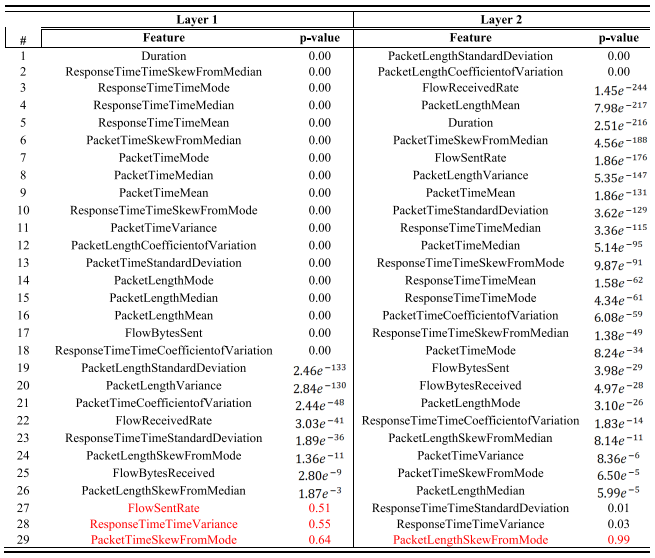
\includegraphics[scale=0.9]{images/behnke_features.PNG}
\centering
\caption{Features listed by Importance, Layer 1 on the Left, Layer 2 on the Right \cite{BehnkeEtAl_FeatureEngineeringMLModelMaliciusDoHTraffic}}
\label{fig:feature_importance}
\end{figure}

\subsection{Three-Layered Approach} \label{3layers}
\cite{MitsuhashiEtAl_IdentifyingmaliciousDNSTunnelTools} developed a system that is able to identify the DNS tunnel tool that is causing the malicious DNS traffic. The basis of this system is shown in the previous works \cite{SinghRoy_DetectingMalicousDoHTrafficML}, \cite{Banadaki_DetectingMalicousDoHTrafficinDNSUsingML}, and \cite{BehnkeEtAl_FeatureEngineeringMLModelMaliciusDoHTraffic}, where the first step is the separation of DoH traffic and normal DNS traffic, and the second step is to detect malicious DoH traffic. \cite{MitsuhashiEtAl_IdentifyingmaliciousDNSTunnelTools} added a third step to that system which is the identification of the malicious DNS tunnel tool, i.e. dns2tcp, dnscat2, and iodine (see Figure \ref{fig:3_layers}). They used the data-set of \cite{montazerishatoori2020anomaly} for their evaluation where they extracted 28 statistical traffic features and chose the machine learning models XGBoost, Light Gradient Boost Machine, and CatBoost to test for the best performing model in each step. The comparison the models in each of the three phases resulted in the selection of XGBoost for the first phase, Light Gradient Boost for the second stage and CatBoost in the third stage due to their performance and accuracy in the respective phase. Moreover, they found that \textit{Mode Packet Length} and \textit{Mean Packet Time} were the most important features for stage one, \textit{Mode Packet Length} and \textit{Median Packet Length} were the most important features for stage two. In the third stage, the most important features followed the pattern \textit{“Request/response time difference”}, and according to that pattern the most important features were \textit{Median Request/response time difference}, \textit{Skew from median Request/response time difference}, \textit{Skew from median Request/response time difference}, and \textit{Skew from mode Request/response time difference}. XGBoost in the first stage had the accuracy of 99.81\%, the precision of 99.81\%, and the F-score of 99.87\%, CatBoost in the second stage had the accuracy of 99.99\%, the precision of 100\%, and the F-score of 99.99\%, and Light Gradient Boost Machine in the third stage had the accuracy of 97.22\%, the precision of 94.97\%, and the F-score of 95.19\%.

\begin{figure} [ht]
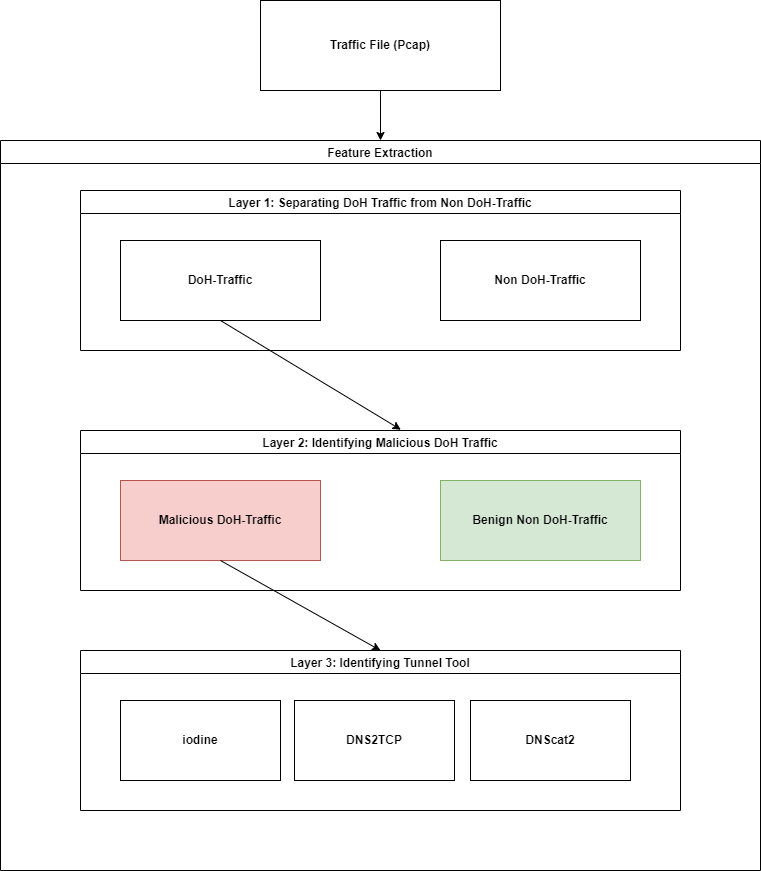
\includegraphics[scale=0.55]{3_layers.png}
\centering
\caption{Illustration of the Three-Layered Approach}
\label{fig:3_layers}
\end{figure}

\section{Deep Learning Based Approach} \label{dl}
\cite{AlFawaRehEtAl_DetectingMaliciousDNSQueriesBRNN} used the deep learning algorithm Bi-Directional Recurrent Neural Network (BRNN) to detect malicious DNS queries over encrypted Tunnels. They used the data-set of \cite{montazerishatoori2020anomaly} for their evaluation, which they pre-processed by deleting redundant or zero rows, then they normalized all the values between a specific range, labelled the values into malicious and benign, and split them into a training and a testing set with the ratio of 80\% to 20\%. From the data set they extracted 34 features but they used only statistical features, therefore they deleted the 6 non-statistical features. In the training phase, they trained their model to identify benign and malicious DoH query patterns, and in the following testing phase they tested if the model was able to identify the trained patterns. They achieved an accuracy of 100\% with no false positives and false negatives rates and concluded that their model is an effective way for organizations to monitor and protect their environment.

\begin{center}
\begin{tabular}{ |c|l| }
\hline
Reference & Key Dimensions \\
\hline
 \cite{HuangEtAl_DoHDowngradeAttack} & Downgrading Attacks on DoH connections\\ 
 \hline
 \cite{Hjelm_ANewNeedle} & Caption of DoH traffic\\
 \hline
 \multirow{2}{*}{\cite{VeshkinEtAl_DoHInsightML}} & Separation of DoH traffic from DNS traffic using Machine Learning Models\\
 & Feature analysis\\
 \hline
 \multirow{2}{*}{\cite{montazerishatoori2020anomaly}} & Feature extraction \\ & Creation of a DoH data-set \\
 \hline
 \cite{SinghRoy_DetectingMalicousDoHTrafficML} & Tests of MLmodels to detect malicious traffic\\
 \hline
 \multirow{2}{*}{\cite{Banadaki_DetectingMalicousDoHTrafficinDNSUsingML}} & Two layered approach for detection of malicious DoH traffic\\
 & Tests of ML models\\
 \hline
 \multirow{3}{*}{\cite{BehnkeEtAl_FeatureEngineeringMLModelMaliciusDoHTraffic}} & Improvement of \cite{Banadaki_DetectingMalicousDoHTrafficinDNSUsingML}'s work\\
 & Statistical tests for feature analysis\\
 & Sequential Forward Selection to find optimal amount of features for ML models\\
 \hline
 \cite{MitsuhashiEtAl_IdentifyingmaliciousDNSTunnelTools} & Three layered approach to find tunnel tool causing malicious DoH traffic\\
 \hline
 \cite{AlFawaRehEtAl_DetectingMaliciousDNSQueriesBRNN} & Use Deep Learning models to detect malicious DoH traffic\\ 
\hline
\end{tabular}
\captionof{table}{Summary of the References presented in this Chapter} \label{tab:summary} 
\end{center}
